\documentclass[aspectratio=169, 11pt]{beamer}

% ── Tema y colores ──
\usetheme{Madrid}
\usecolortheme{default}

\definecolor{mainblue}{HTML}{0D47A1}
\definecolor{medblue}{HTML}{1E88E5}
\definecolor{accentgreen}{HTML}{2E7D32}
\definecolor{darkgray}{HTML}{333333}
\definecolor{lightgray}{HTML}{757575}

\setbeamercolor{structure}{fg=mainblue}
\setbeamercolor{palette primary}{bg=mainblue, fg=white}
\setbeamercolor{palette secondary}{bg=medblue, fg=white}
\setbeamercolor{palette tertiary}{bg=mainblue!80, fg=white}
\setbeamercolor{frametitle}{bg=mainblue, fg=white}
\setbeamercolor{title}{fg=white}
\setbeamercolor{subtitle}{fg=white!85}
\setbeamercolor{item}{fg=mainblue}
\setbeamercolor{block title}{bg=mainblue, fg=white}
\setbeamercolor{block body}{bg=mainblue!5}

\setbeamerfont{title}{size=\Large, series=\bfseries}
\setbeamerfont{frametitle}{size=\large, series=\bfseries}
\setbeamerfont{subtitle}{size=\normalsize}

% Quitar barra de navegación
\setbeamertemplate{navigation symbols}{}
% Números de slide en footer
\setbeamertemplate{footline}{
    \hfill\insertframenumber/\inserttotalframenumber\hspace{0.5cm}\vspace{0.3cm}
}

% ── Paquetes ──
\usepackage[utf8]{inputenc}
\usepackage[T1]{fontenc}
\usepackage[spanish]{babel}
\usepackage{graphicx}
\usepackage{tikz}
\usetikzlibrary{positioning, arrows.meta, fit, backgrounds, calc, decorations.pathmorphing}
\usepackage{booktabs}
\usepackage{multicol}

\graphicspath{{images/}}

% ── Metadata ──
\title[DeepSolation]{Clasificación de Daño en Aisladores Sísmicos\\mediante Machine Learning y Deep Learning}
\subtitle{Un Análisis Comparativo con Señales de Vibración Ambiental}
\author{Tesis de Maestría en Data Science e Inteligencia Artificial}
\institute{Universidad de Ingeniería y Tecnología --- UTEC}
\date{2026}

% ════════════════════════════════════════════════════════════════
\begin{document}

% ── SLIDE 1: PORTADA ──
{
\setbeamercolor{background canvas}{bg=mainblue}
\begin{frame}[plain]
    \vspace{1.5cm}
    \begin{center}
        {\usebeamerfont{title}\usebeamercolor[fg]{title}\inserttitle\par}
        \vspace{0.4cm}
        {\usebeamerfont{subtitle}\usebeamercolor[fg]{subtitle}\insertsubtitle\par}
        \vspace{1.2cm}
        {\color{white!85}\insertauthor\par}
        \vspace{0.3cm}
        {\color{white!70}\small\insertinstitute\par}
        \vspace{0.3cm}
        {\color{white!60}\small\insertdate\par}
    \end{center}
\end{frame}
}


% ── SLIDE 2: PROBLEMA Y MOTIVACIÓN ──
\begin{frame}{Problema y Motivación}
    \begin{itemize}
        \setlength\itemsep{0.5em}
        \item Perú se ubica en el Cinturón de Fuego del Pacífico --- alta actividad sísmica
        \item Los aisladores sísmicos (LRB) protegen edificios críticos, pero se degradan con el tiempo
        \item La inspección actual es \textbf{visual y manual}:
        \begin{itemize}
            \item Costosa, subjetiva, requiere especialistas certificados
            \item No detecta daño interno (degradación del núcleo de plomo)
        \end{itemize}
        \item Las vibraciones ambientales (microtremores) son señales \textbf{no invasivas}, medibles 24/7
        \item \textbf{Pregunta de investigación:}
        \begin{itemize}
            \item ¿Se puede clasificar automáticamente el daño en aisladores usando ML/DL sobre señales de vibración?
        \end{itemize}
    \end{itemize}
\end{frame}


% ── SLIDE 3: OBJETIVOS ──
\begin{frame}{Objetivos de la Investigación}
    \begin{block}{Objetivo General}
        Desarrollar y comparar pipelines de ML y DL para clasificar el nivel de daño en aisladores sísmicos a partir de señales de vibración ambiental.
    \end{block}
    \vspace{0.3cm}
    \begin{enumerate}
        \setlength\itemsep{0.3em}
        \item[\textbf{OE1:}] Comparar representaciones espectrales (FFT, CWT, WST, MOMENT, Raw)
        \item[\textbf{OE2:}] Evaluar combinaciones de extracción (PCA, AE) y clasificación (SVM, RF, CNN)
        \item[\textbf{OE3:}] Explorar enfoques alternativos (modelo fundacional, Vision Transformer)
        \item[\textbf{OE4:}] Implementar validación anti-\textit{data leakage} (StratifiedGroupKFold)
        \item[\textbf{OE5:}] Analizar interpretabilidad del modelo CNN con Eigen-CAM
        \item[\textbf{OE6:}] Proponer arquitectura de despliegue productivo
    \end{enumerate}
\end{frame}


% ── SLIDE 4: DATASET ──
\begin{frame}{Dataset: Aisladores Sísmicos Instrumentados}
    \begin{columns}[T]
        \begin{column}{0.52\textwidth}
            \begin{itemize}
                \setlength\itemsep{0.4em}
                \item \textbf{85 aisladores} LRB en 3 edificios del campus de UTEC
                \item 248 mediciones totales (múltiples pasadas por aislador)
                \item 2 sensores por aislador: S1 (base) + S2 (superior)
                \item 3 ejes de aceleración: N-S, E-W, U-D --- 100~Hz
                \item Clasificación \textbf{binaria}:
                \begin{itemize}
                    \item Sin Daño (N1): 48 aisladores (56.5\%)
                    \item Con Daño (N2+N3): 37 aisladores (43.5\%)
                \end{itemize}
                \item 82 para train/val, 3 reservados para test
            \end{itemize}
        \end{column}
        \begin{column}{0.45\textwidth}
            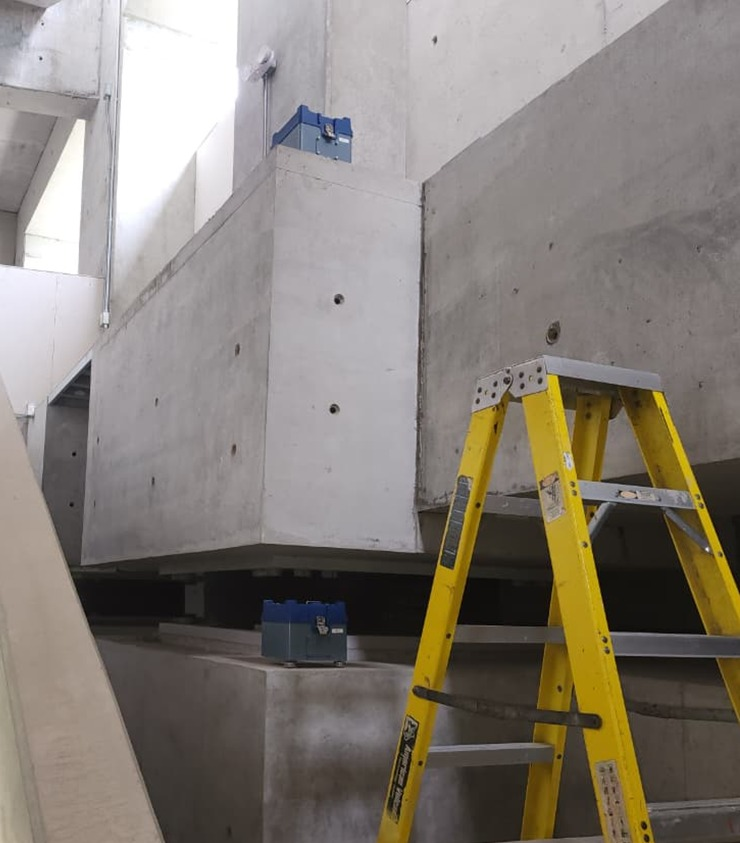
\includegraphics[width=\textwidth]{cap3_medicion_aislador_utec.jpeg}
        \end{column}
    \end{columns}
\end{frame}


% ── SLIDE 5: EXPLORACIÓN ──
\begin{frame}{Exploración: Espectros FFT y Clustering}
    \begin{columns}[T]
        \begin{column}{0.48\textwidth}
            \begin{itemize}
                \setlength\itemsep{0.5em}
                \item Los espectros FFT muestran diferencias \textbf{sutiles} entre niveles de daño
                \item Clustering K-Means ($k=3$) sobre PCA:
                \begin{itemize}
                    \item Las clases de daño \textbf{no} son separables de forma naïve
                    \item Los clusters se alinean más con el \textbf{edificio} que con el daño
                \end{itemize}
                \item Justifica el uso de \textbf{modelos supervisados}
            \end{itemize}
        \end{column}
        \begin{column}{0.50\textwidth}
            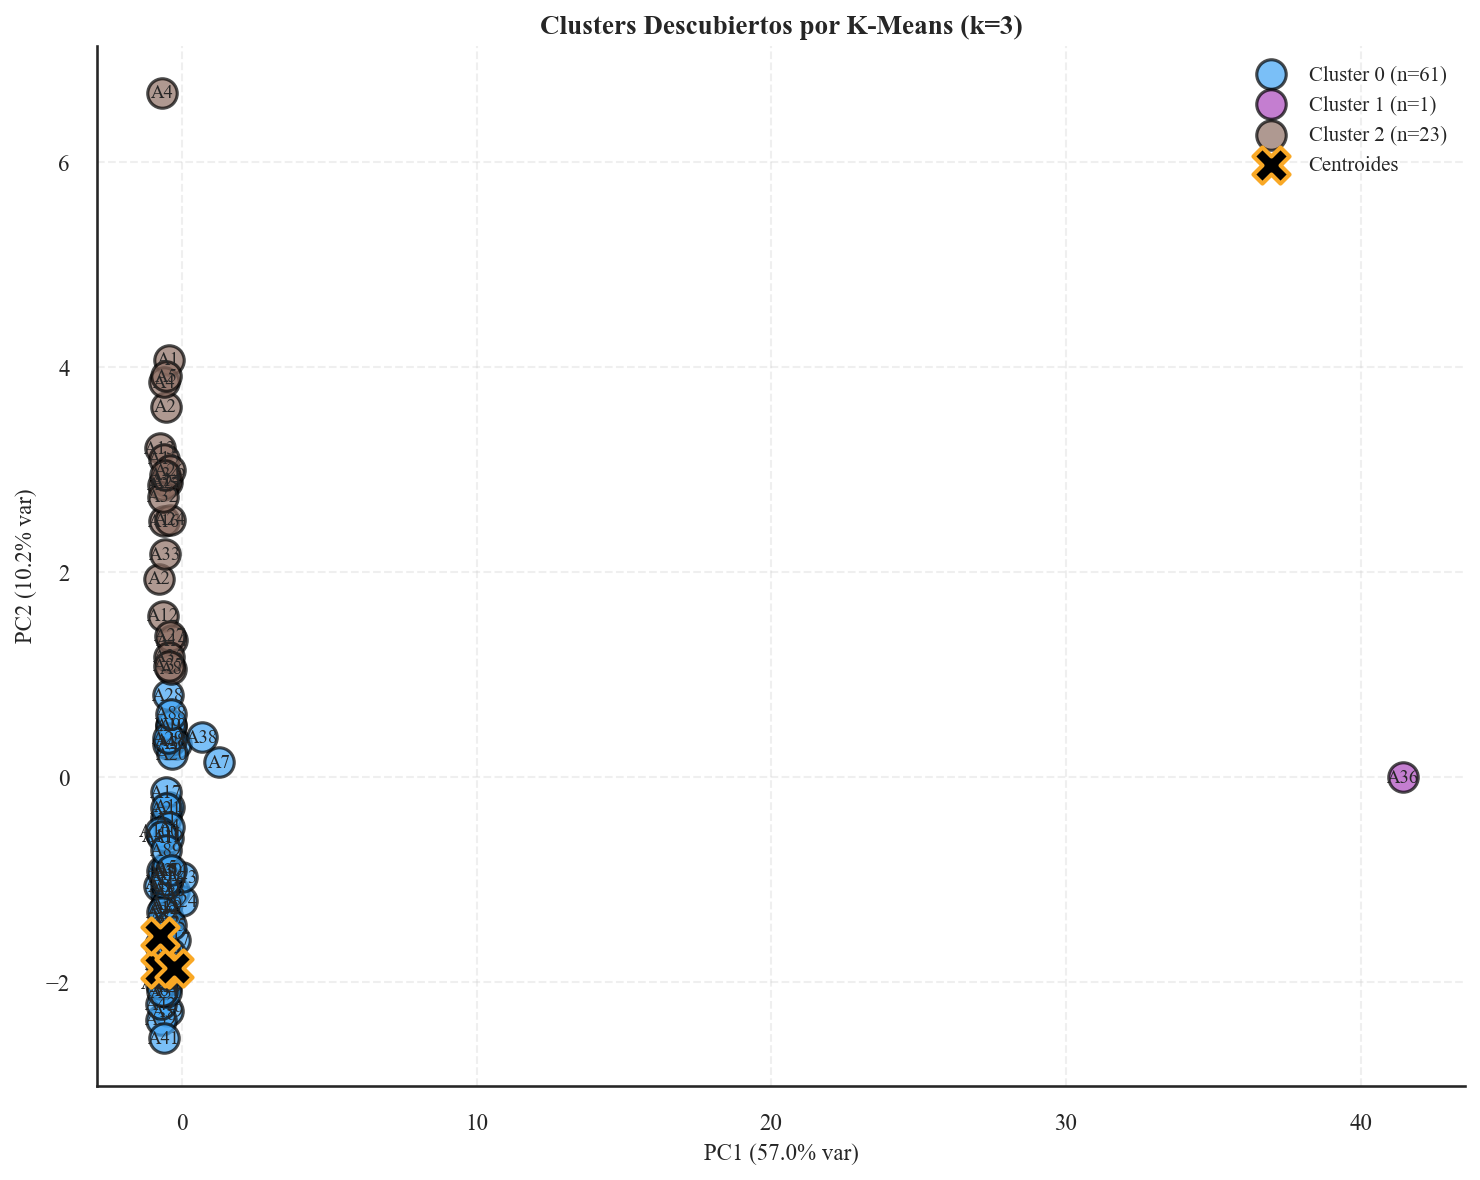
\includegraphics[width=\textwidth]{cap4_clustering_pca_kmeans.png}
        \end{column}
    \end{columns}
\end{frame}


% ── SLIDE 6: REPRESENTACIONES (TikZ) ──
\begin{frame}[plain]
    \centering
    \resizebox{0.92\textwidth}{!}{
        \input{diagrama_representaciones_content.tex}
    }
\end{frame}


% ── SLIDE 7: 12 PIPELINES (TikZ) ──
\begin{frame}[plain]
    \centering
    \resizebox{0.88\textwidth}{!}{
        \begin{tikzpicture}[
    % Estilos de nodos
    repr/.style={
        rectangle, rounded corners=4pt, draw=#1, fill=#1!12,
        minimum width=3.8cm, minimum height=0.9cm,
        font=\sffamily\small\bfseries, text=black, align=center,
        line width=0.8pt
    },
    extr/.style={
        rectangle, rounded corners=4pt, draw=#1, fill=#1!12,
        minimum width=3.8cm, minimum height=0.9cm,
        font=\sffamily\small\bfseries, text=black, align=center,
        line width=0.8pt
    },
    clas/.style={
        rectangle, rounded corners=4pt, draw=#1, fill=#1!12,
        minimum width=3.2cm, minimum height=0.9cm,
        font=\sffamily\small\bfseries, text=black, align=center,
        line width=0.8pt
    },
    stage label/.style={
        font=\sffamily\large\bfseries, text=#1
    },
    arrow/.style={
        -{Stealth[length=5pt, width=4pt]}, line width=0.7pt, color=#1
    },
    group box/.style={
        rounded corners=8pt, draw=#1!50, fill=#1!4,
        line width=1pt, dashed
    }
]

% ── Definir colores ──
\definecolor{rawgray}{HTML}{757575}
\definecolor{fftblue}{HTML}{1565C0}
\definecolor{cwtgreen}{HTML}{2E7D32}
\definecolor{wstgreen}{HTML}{388E3C}
\definecolor{momorange}{HTML}{F57C00}
\definecolor{pcaamber}{HTML}{FF8F00}
\definecolor{aeindigo}{HTML}{5C6BC0}
\definecolor{dirteal}{HTML}{00897B}
\definecolor{svmred}{HTML}{C62828}
\definecolor{rfgreen}{HTML}{2E7D32}
\definecolor{cnnpurp}{HTML}{8E24AA}
\definecolor{swinteal}{HTML}{00695C}

% ════════════════════════════════════════
% STAGE 1: Representaciones (columna izq)
% ════════════════════════════════════════
\node[repr=rawgray]   (raw)  at (0, 0)    {Raw (señal cruda)};
\node[repr=fftblue]   (fft)  at (0, -1.4) {FFT (log-magnitud)};
\node[repr=cwtgreen]  (cwt)  at (0, -2.8) {CWT (escalogramas)};
\node[repr=wstgreen]  (wst)  at (0, -4.2) {WST (scattering)};
\node[repr=momorange] (mom)  at (0, -5.6) {MOMENT (embeddings)};

% ════════════════════════════════════════
% STAGE 2: Extracción (columna central)
% ════════════════════════════════════════
\node[extr=pcaamber]  (pca)  at (6.5, -0.7)  {Reducción Lineal (PCA)};
\node[extr=aeindigo]  (ae)   at (6.5, -2.8)  {Autoencoder Conv 1D};
\node[extr=dirteal]   (dir)  at (6.5, -4.9)  {Directo};

% ════════════════════════════════════════
% STAGE 3: Clasificación (columna derecha)
% ════════════════════════════════════════
\node[clas=svmred]   (svm1)  at (12.5, 0.3)   {SVM};
\node[clas=rfgreen]  (rf1)   at (12.5, -0.7)  {Random Forest};
\node[clas=svmred]   (svm2)  at (12.5, -1.7)  {SVM};
\node[clas=rfgreen]  (rf2)   at (12.5, -2.7)  {Random Forest};
\node[clas=cnnpurp]  (cnn)   at (12.5, -3.7)  {CNN Head};
\node[clas=swinteal] (swin)  at (12.5, -4.7)  {Swin-Tiny};
\node[clas=svmred]   (svm3)  at (12.5, -5.7)  {SVM};
\node[clas=rfgreen]  (rf3)   at (12.5, -6.7)  {Random Forest};

% ════════════════════════════════════════
% FLECHAS Stage 1 → Stage 2
% ════════════════════════════════════════
% Raw → PCA
\draw[arrow=rawgray]  (raw.east)  -- (pca.west);
% FFT → PCA y AE
\draw[arrow=fftblue]  (fft.east)  -- (pca.west);
\draw[arrow=fftblue]  (fft.east)  -- (ae.west);
% CWT → Directo
\draw[arrow=cwtgreen] (cwt.east)  -- (dir.west);
% WST → Directo
\draw[arrow=wstgreen] (wst.east)  -- (dir.west);
% MOMENT → Directo
\draw[arrow=momorange](mom.east)  -- (dir.west);

% ════════════════════════════════════════
% FLECHAS Stage 2 → Stage 3
% ════════════════════════════════════════
% PCA → SVM, RF (raw + fft comparten salida)
\draw[arrow=pcaamber] (pca.east)  -- (svm1.west);
\draw[arrow=pcaamber] (pca.east)  -- (rf1.west);
% AE → SVM, RF, CNN
\draw[arrow=aeindigo] (ae.east)   -- (svm2.west);
\draw[arrow=aeindigo] (ae.east)   -- (rf2.west);
\draw[arrow=aeindigo] (ae.east)   -- (cnn.west);
% Directo → Swin, SVM, RF
\draw[arrow=dirteal]  (dir.east)  -- (swin.west);
\draw[arrow=dirteal]  (dir.east)  -- (svm3.west);
\draw[arrow=dirteal]  (dir.east)  -- (rf3.west);

% ════════════════════════════════════════
% ETIQUETAS de pipeline (derecha)
% ════════════════════════════════════════
\node[right=0.3cm of svm1, font=\sffamily\scriptsize, text=rawgray]  {Raw+PCA+SVM};
\node[right=0.3cm of rf1,  font=\sffamily\scriptsize, text=rawgray]  {Raw+PCA+RF};
\node[right=0.3cm of svm2, font=\sffamily\scriptsize, text=aeindigo] {FFT+AE+SVM};
\node[right=0.3cm of rf2,  font=\sffamily\scriptsize, text=aeindigo] {FFT+AE+RF};
\node[right=0.3cm of cnn,  font=\sffamily\scriptsize, text=cnnpurp]  {FFT+AE+CNN};
\node[right=0.3cm of swin, font=\sffamily\scriptsize, text=swinteal] {CWT+Swin-Tiny};
\node[right=0.3cm of svm3, font=\sffamily\scriptsize, text=dirteal]  {WST/MOM+SVM};
\node[right=0.3cm of rf3,  font=\sffamily\scriptsize, text=dirteal]  {WST/MOM+RF};

% ════════════════════════════════════════
% ETIQUETAS de stage (arriba)
% ════════════════════════════════════════
\node[stage label=fftblue]  at (0,    2.0) {Stage 1: Representación};
\node[stage label=pcaamber] at (6.5,  2.0) {Stage 2: Extracción};
\node[stage label=rfgreen]  at (12.5, 2.0) {Stage 3: Clasificación};

% ════════════════════════════════════════
% CAJAS de agrupación (fondo)
% ════════════════════════════════════════
\begin{scope}[on background layer]
    \node[group box=fftblue,
          fit=(raw)(mom), inner sep=12pt] {};
    \node[group box=pcaamber,
          fit=(pca)(dir), inner sep=12pt] {};
    \node[group box=rfgreen,
          fit=(svm1)(rf3), inner sep=12pt] {};
\end{scope}

% ════════════════════════════════════════
% NOTA al pie: total pipelines
% ════════════════════════════════════════
\node[font=\sffamily\small, text=black!60, align=center]
    at (6.5, -8.4)
    {12 pipelines evaluados bajo las mismas condiciones de validación cruzada (StratifiedGroupKFold, 5 folds)};

\end{tikzpicture}
    }
\end{frame}


% ── SLIDE 8: RESULTADOS RANKING ──
\begin{frame}{Resultados: Ranking de los 12 Pipelines}
    \centering
    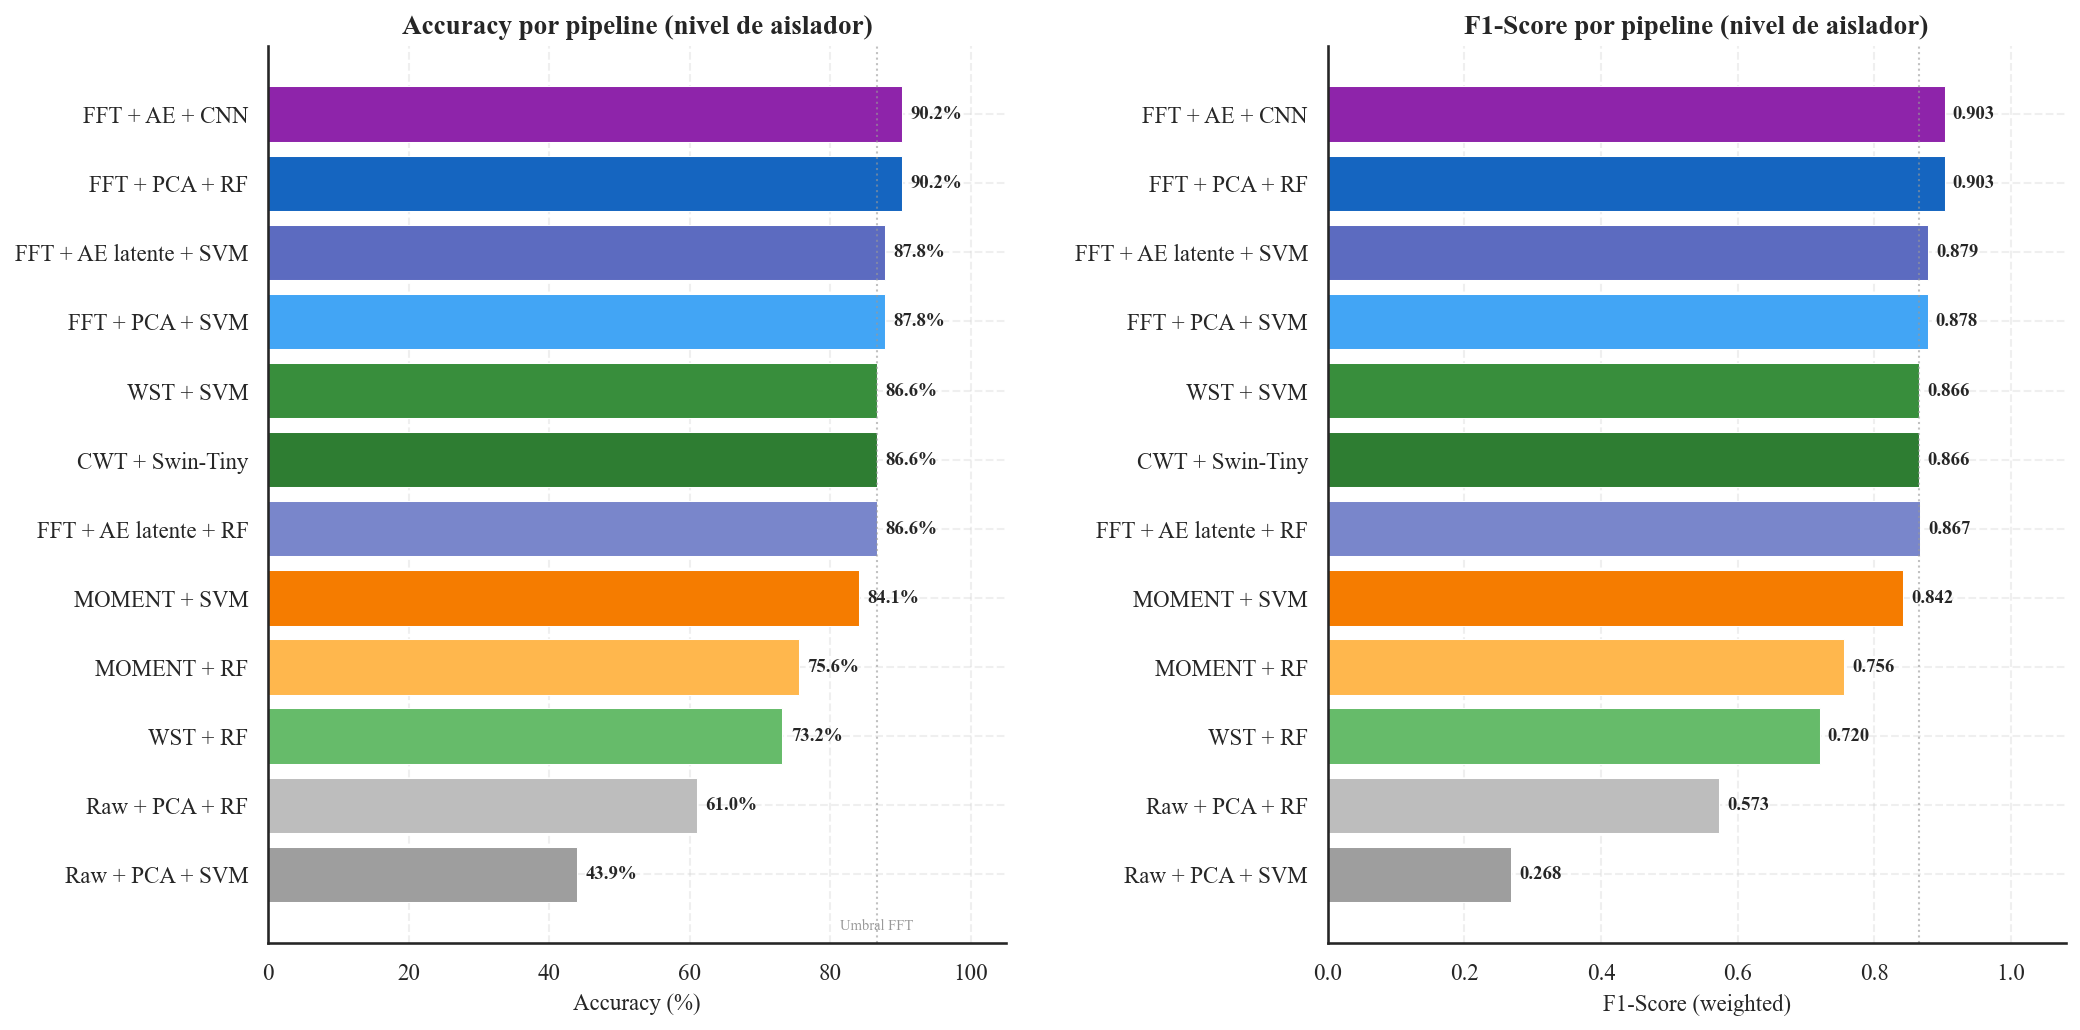
\includegraphics[width=0.95\textwidth]{cap4_accuracy_f1_barras.png}
\end{frame}


% ── SLIDE 9: SENSIBILIDAD CLÍNICA ──
\begin{frame}{Sensibilidad Clínica: ¿Cuánto daño detectamos?}
    \begin{columns}[T]
        \begin{column}{0.48\textwidth}
            \begin{itemize}
                \setlength\itemsep{0.5em}
                \item \textbf{FFT + PCA + RF:}
                \begin{itemize}
                    \item Recall = \textbf{97.2\%}
                    \item Solo 1 falso negativo de 36 dañados
                \end{itemize}
                \item En seguridad estructural, \textbf{no detectar daño} es mucho más costoso que una falsa alarma
                \item Los 4 mejores pipelines superan 94\% de Recall
            \end{itemize}
        \end{column}
        \begin{column}{0.50\textwidth}
            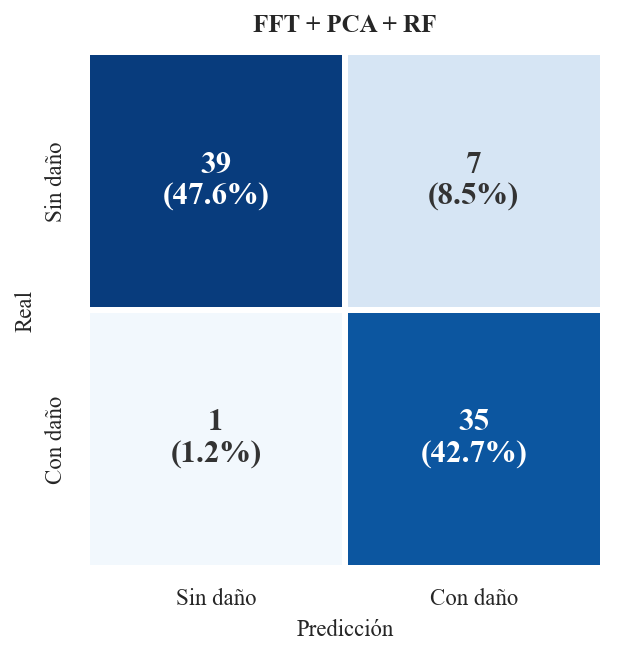
\includegraphics[width=\textwidth]{cap4_cm_fft_pca_rf_fold_global_isolator.png}
        \end{column}
    \end{columns}
\end{frame}


% ── SLIDE 10: EFICIENCIA COMPUTACIONAL ──
\begin{frame}{Eficiencia Computacional}
    \begin{columns}[T]
        \begin{column}{0.45\textwidth}
            \begin{itemize}
                \setlength\itemsep{0.4em}
                \item \textbf{FFT + PCA + RF:}
                \begin{itemize}
                    \item 24 segundos de entrenamiento
                    \item 116~ms de inferencia
                \end{itemize}
                \item \textbf{FFT + AE + CNN:}
                \begin{itemize}
                    \item 27 minutos de entrenamiento
                    \item 13~ms de inferencia (9x más rápido)
                \end{itemize}
                \item \textit{Trade-off}: RF práctico para reentrenamiento; AE+CNN más ágil en producción
            \end{itemize}
        \end{column}
        \begin{column}{0.53\textwidth}
            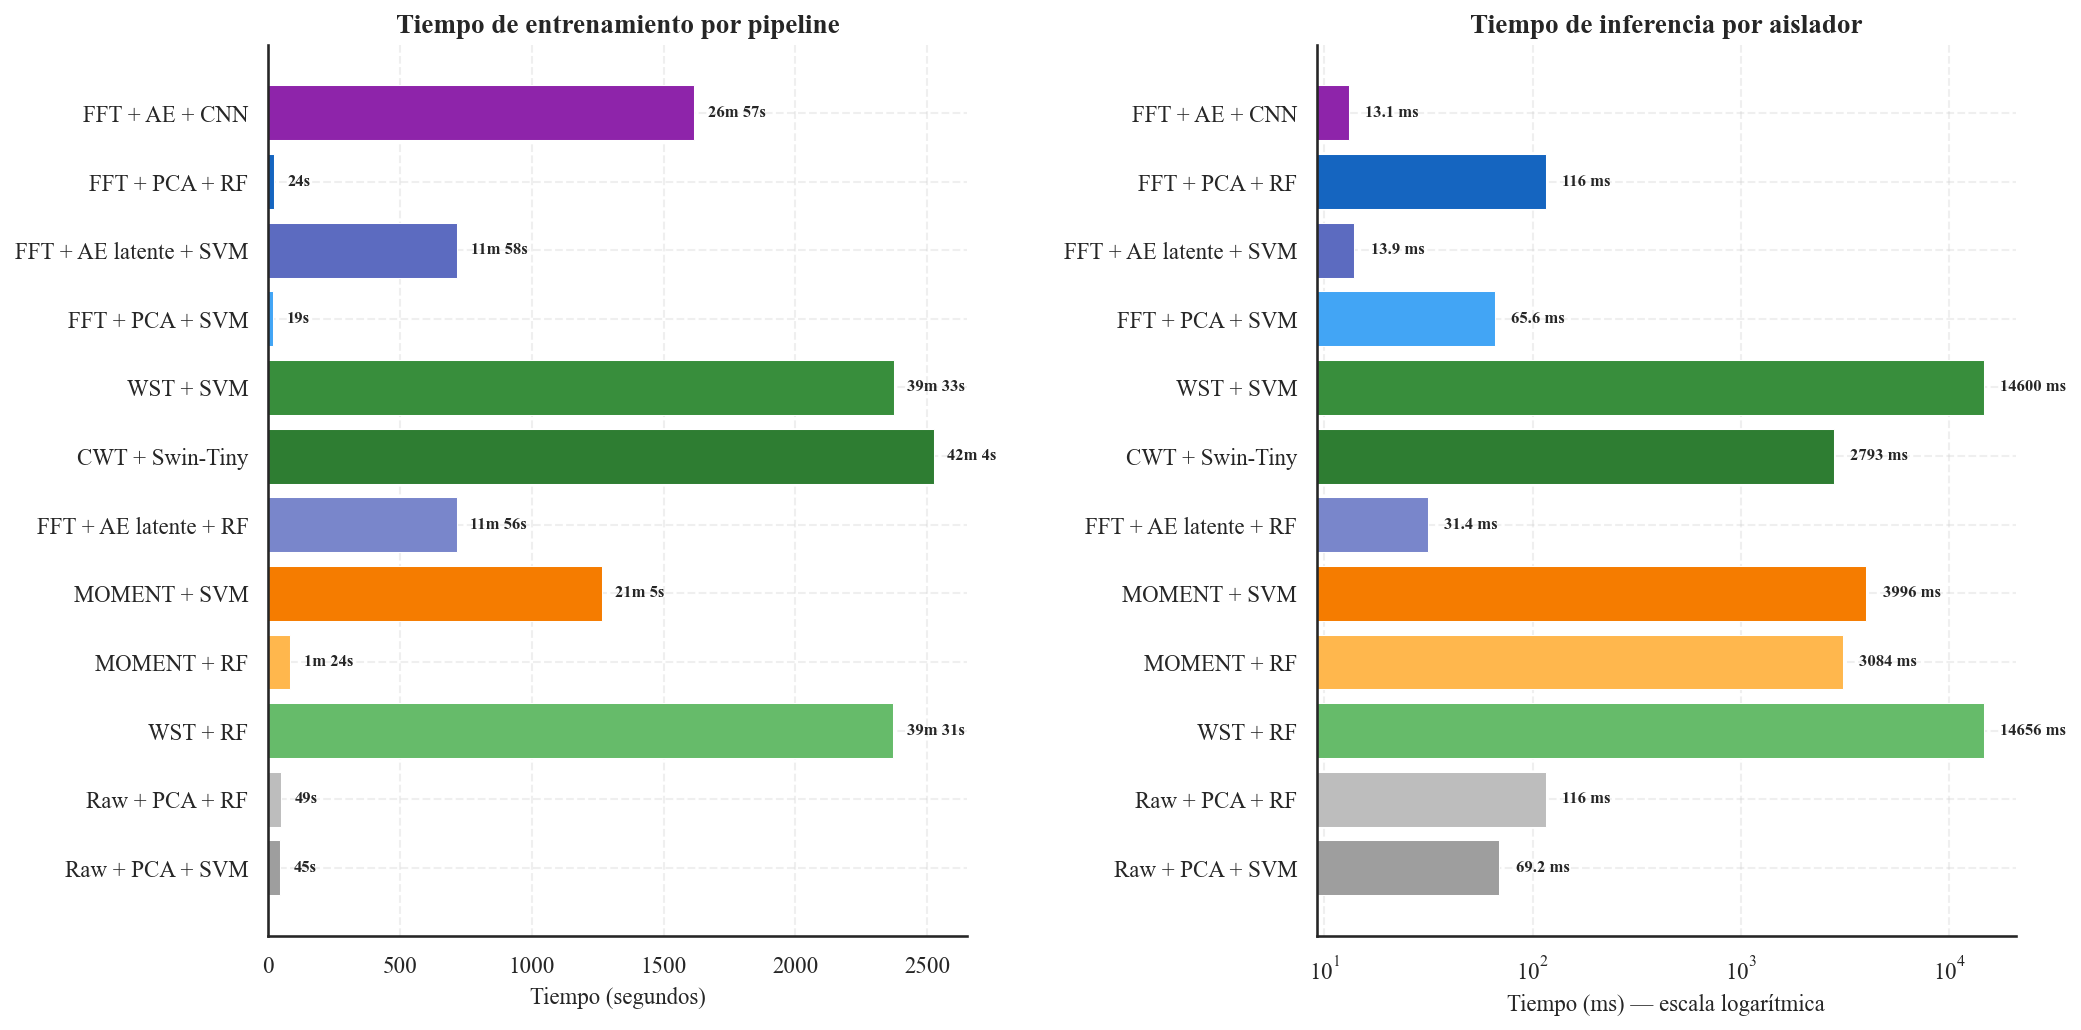
\includegraphics[width=\textwidth]{cap4_tiempos_training_inferencia.png}
        \end{column}
    \end{columns}
\end{frame}


% ── SLIDE 11: HYPERPARAMETER TUNING ──
\begin{frame}{Optimización de Hiperparámetros}
    \begin{itemize}
        \setlength\itemsep{0.4em}
        \item \textbf{FFT + PCA + RF/SVM} (RandomizedSearchCV, 50 iteraciones):
        \begin{itemize}
            \item RF tuneado: 87.8\% --- \textbf{peor} que el original (90.2\%)
            \item Los defaults de sklearn ya son óptimos para este dataset
        \end{itemize}
        \item \textbf{FFT + AE + CNN} (random search, 25 iteraciones):
        \begin{itemize}
            \item Mejora marginal: 90.2\% $\rightarrow$ 91.5\% (+1.3\%)
            \item Hallazgo: ReLU $>$ LeakyReLU, fine-tuning perjudica (overfitting)
        \end{itemize}
    \end{itemize}
    \vspace{0.5cm}
    \begin{block}{Conclusión clave}
        El techo de rendimiento está limitado por el \textbf{tamaño del dataset} (82 aisladores), no por los hiperparámetros. \textbf{Más datos $>$ mejor tuning.}
    \end{block}
\end{frame}


% ── SLIDE 12: INTERPRETABILIDAD EIGEN-CAM ──
\begin{frame}{Interpretabilidad: Eigen-CAM}
    \begin{columns}[T]
        \begin{column}{0.45\textwidth}
            \begin{itemize}
                \setlength\itemsep{0.5em}
                \item ¿Qué frecuencias mira el modelo para decidir?
                \item A nivel individual: alta variabilidad, no distinguible visualmente
                \item Al promediar 70 aisladores por clase:
                \begin{itemize}
                    \item Banda \textbf{10--13~Hz}: mayor activación en aisladores sanos
                    \item Resonancia natural del LRB intacto
                \end{itemize}
                \item El modelo detecta \textbf{normalidad}, no una ``firma de daño''
            \end{itemize}
        \end{column}
        \begin{column}{0.53\textwidth}
            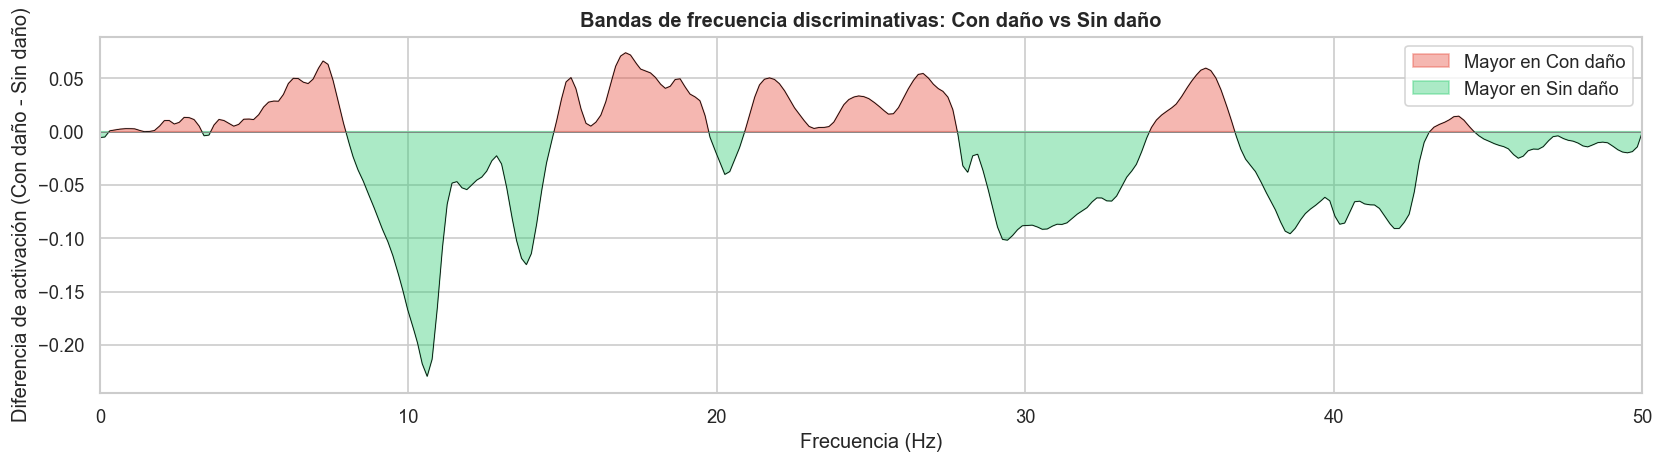
\includegraphics[width=\textwidth]{cap4_eigencam_frecuencias.png}
        \end{column}
    \end{columns}
\end{frame}


% ── SLIDE 13: RADAR MULTIDIMENSIONAL ──
\begin{frame}{Perfil Multidimensional de los Pipelines}
    \centering
    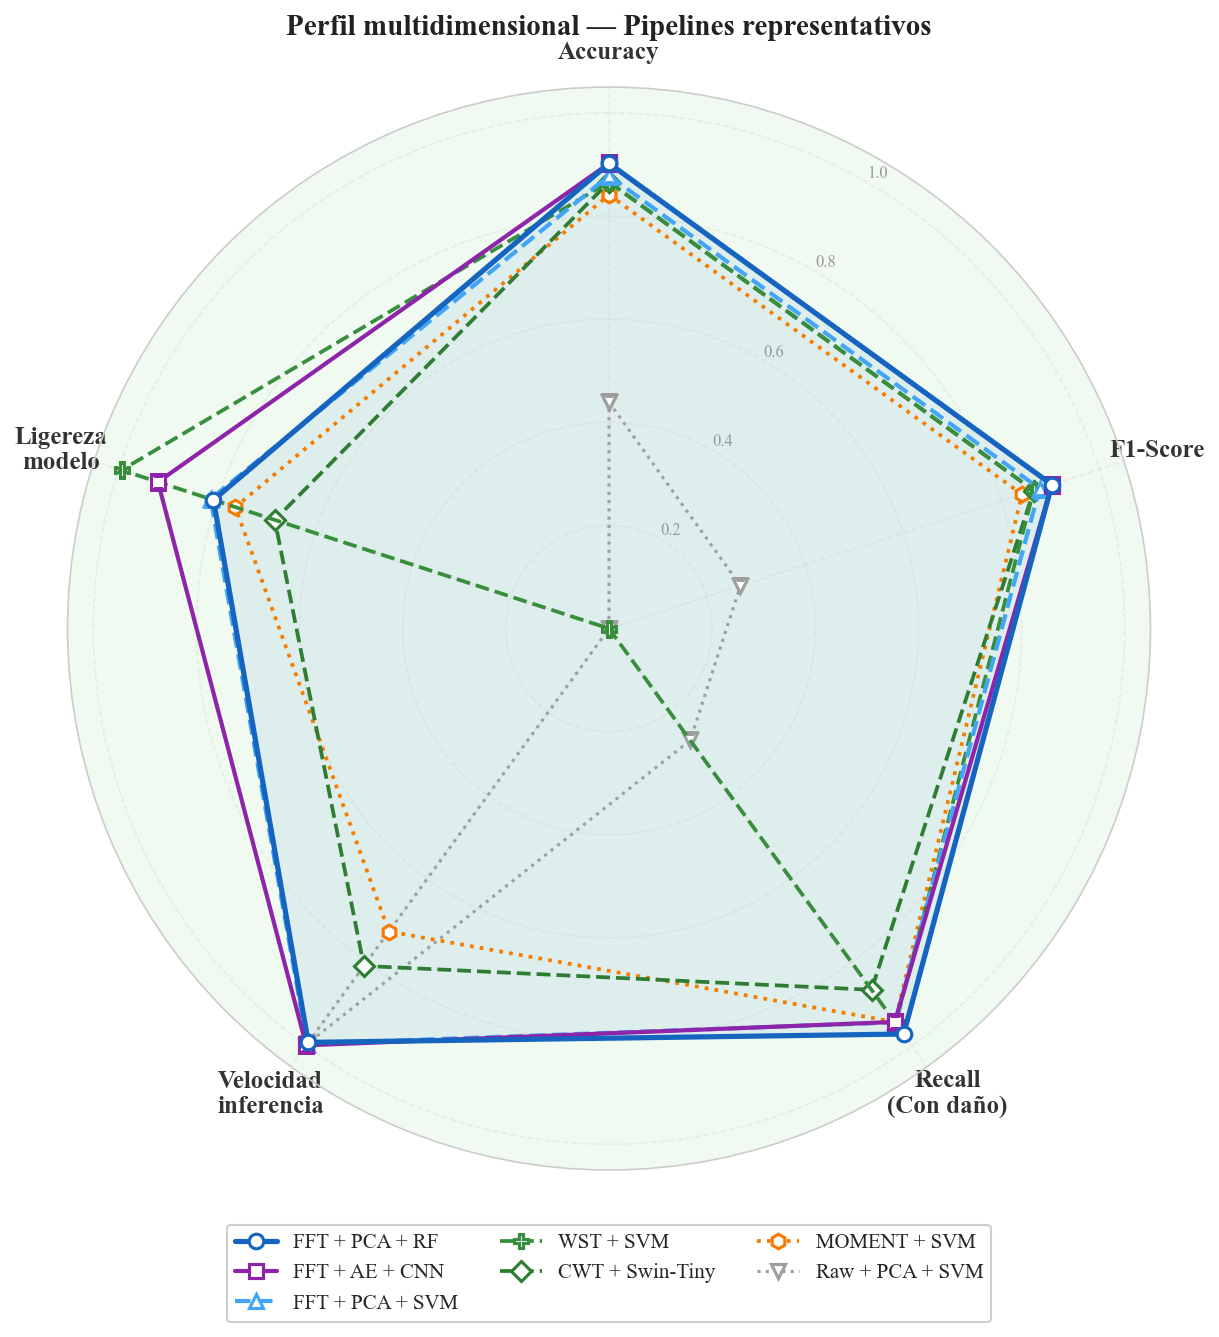
\includegraphics[height=0.85\textheight]{cap4_radar_pipelines.png}
\end{frame}


% ── SLIDE 14: CONCLUSIONES ──
\begin{frame}{Conclusiones}
    \begin{itemize}
        \setlength\itemsep{0.5em}
        \item La \textbf{FFT domina}: los 6 mejores pipelines la usan como representación base
        \begin{itemize}
            \item 44 puntos porcentuales sobre señales crudas (90.2\% vs 43.9\%)
        \end{itemize}
        \item \textbf{ML clásico = Deep Learning} con 82 aisladores
        \begin{itemize}
            \item FFT+PCA+RF y FFT+AE+CNN empatan en 90.2\%
        \end{itemize}
        \item \textbf{Recall de 97.2\%}: viable para screening de seguridad estructural
        \begin{itemize}
            \item Solo 1 falso negativo de 36 aisladores dañados
        \end{itemize}
        \item El autoencoder tiene mayor \textbf{potencial de escalamiento}
        \begin{itemize}
            \item Inferencia 9x más rápida (13~ms vs 116~ms)
        \end{itemize}
        \item Eigen-CAM: la banda \textbf{10--13~Hz} (resonancia LRB) es el marcador clave
    \end{itemize}
\end{frame}


% ── SLIDE 15: LIMITACIONES Y TRABAJO FUTURO ──
\begin{frame}{Limitaciones y Trabajo Futuro}
    \begin{columns}[T]
        \begin{column}{0.48\textwidth}
            \textbf{\color{mainblue}Limitaciones}
            \begin{itemize}
                \setlength\itemsep{0.3em}
                \item Variable de confusión (edificio): los clusters se alinean con el edificio
                \item Dataset pequeño: 82 aisladores limita el DL
                \item Solo clasificación binaria: insuficientes muestras N3
            \end{itemize}
        \end{column}
        \begin{column}{0.48\textwidth}
            \textbf{\color{accentgreen}Trabajo Futuro}
            \begin{itemize}
                \setlength\itemsep{0.3em}
                \item Incorporar aisladores de otras locaciones geográficas
                \item Escalar dataset para que DL supere a ML
                \item Clasificación multiclase (N1/N2/N3)
                \item Prototipo de despliegue para monitoreo continuo
            \end{itemize}
        \end{column}
    \end{columns}
\end{frame}


% ── SLIDE 16: CIERRE ──
{
\setbeamercolor{background canvas}{bg=mainblue}
\begin{frame}[plain]
    \vspace{2cm}
    \begin{center}
        {\Huge\color{white}\bfseries ¡Gracias!\par}
        \vspace{0.8cm}
        {\color{white!85}\large Clasificación de Daño en Aisladores Sísmicos\\mediante Machine Learning y Deep Learning\par}
        \vspace{1cm}
        {\color{white!70}\Large ¿Preguntas?\par}
    \end{center}
\end{frame}
}

\end{document}
